
\documentclass{beamer}
\usepackage{amsmath}
\usepackage{graphicx}

\title{Maxima using Gradient Ascent for $f(x) = \frac{\log{x}}{x}$}
\author{EE24BTECH11012 - Bhavanisankar G S}
\date{\today}

\begin{document}

\frame{\titlepage}

\begin{frame}
\frametitle{Question}
\textbf{Show that the function} $f(x) = \frac{\log{x}}{x}$ \textbf{has a maximum at} $x = e$.
\end{frame}

\begin{frame}
\frametitle{Theoretical Solution}
Given function: $y(x) = \frac{\log{x}}{x}$ \\[0.2cm]
First derivative: $y'(x) = \frac{1 - \log{x}}{x^2}$ \\[0.2cm]
Second derivative: $y''(x) = \frac{2 \log{x} - 3}{x^3}$\\[0.2cm]
Critical points: Solve $y'(x) = 0 \Rightarrow x = e$ \\[0.2cm]
Double derivative test: $y''(e) = \frac{-1}{e^3} < 0 \Rightarrow$ Maximum at $x = e$
\end{frame}

\begin{frame}
\frametitle{Computational Solution}
Using Gradient Ascent: \\[0.2cm]
Iteration formula: $x_{n+1} = x_n + \alpha f'(x_n)$ \\[0.2cm]
		   $x_{n+1} = x_{n} + \alpha \left( {\frac{1 - \log{x_{n}}}{x_{n}^2}} \right)$ \\[0.2cm]
With $\alpha = 0.001$: \\[0.2cm]
$x_{\text{max}} = 2.717779896744937$ \\
$y_{\text{max}} = 0.36787943489794817$
\end{frame}

\begin{frame}
\frametitle{Graphical Representation}
\begin{center}
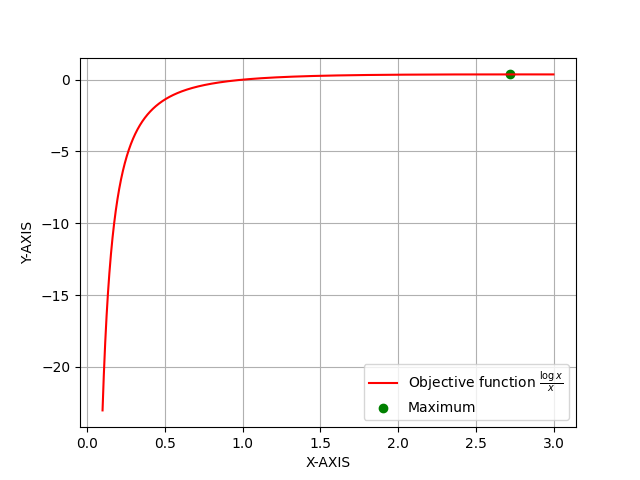
\includegraphics[width=0.7\textwidth]{fig.png} \\
\textit{Plot of the function $f(x) = \frac{\log{x}}{x}$}
\end{center}
\end{frame}

\end{document}
